\documentclass[e2_tp1_main.tex]{subfiles}

\begin{document}

\section{Análisis de la protección}
Se decidió utilizar una protección foldback dado que esta evita el pasarnos de la corriente de salida máxima establecida, $Io_{m\acute{a}x}=1.5\thinspace{A}$ y nos limita la cantidad de potencia a disipar por una menor a la dada por una protección lineal reduciendo costos.
Al agregar la protección foldback nos quedamos con el siguiente circuito:
\begin{figure}[H]
  \centering
   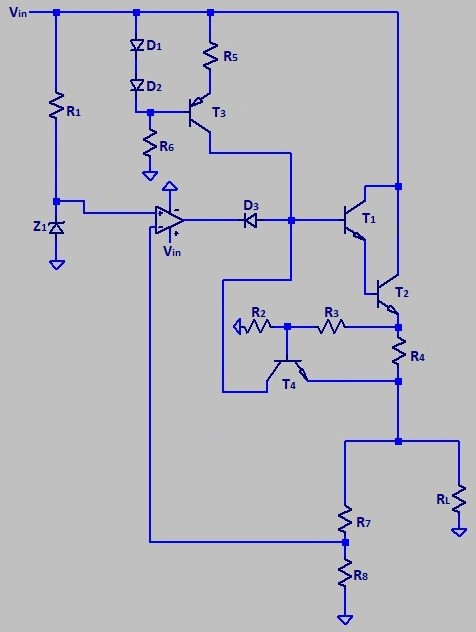
\includegraphics[width=0.5\textwidth]{CircuitoProtec.jpg}
   \caption{Circuito con protección}
   \label{fig:CircuitoProtec}
\end{figure}
De la figura ~\ref{fig:CircuitoProtec} podemos observar que la protección va a tener los siguientes parámetros:
\begin{figure}[H]
  \centering
   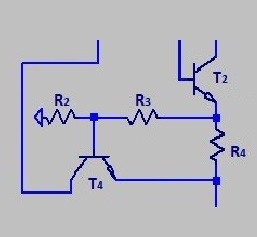
\includegraphics[width=0.5\textwidth]{AnalProtec.jpg}
   \caption{Análisis del circuito}
   \label{fig:AnalProtec}
\end{figure}
De la ~\ref{fig:AnalProtec} al recorrer la malla marcada obtenemos la siguiente ecuación:
$$(I_o - I_{e4})R_4=V_{be}+\frac{V_0+(I_o - I_{e4})R_4}{R_2+R_3}R_3$$
Dado que la corriente $I_{e4}$ es la corriente que viene de la fuente de corriente y debido a que la corriente $I_o$ es dado por $\beta_1\beta_2$ podemos despreciar la corriente $I_{e4}$ dando como resultado la siguiente ecuación:
$$I_oR_4=V_{be}+\frac{V_0+I_oR_4}{R_2+R_3}R_3$$
Para la elección de los componentes se fijaron los componentes $R_3$ y $R_4$ de forma tal que el componente $R_2$ se elige a partir del siguiente despeje:
$$R_2=\frac{(V_o+I_OR_4)R3}{I_0R_4-V_{be}}R_3-R_3$$
Se despejo el valor de $R_2$ utilizando las siguientes condiciones:
\begin{table}[H]
	\begin{center}
		\begin{tabular}{|c|c|}
			\hline
			Elemento & Valor\\
			\hline
			$R_4$ & $0.6\!\Omega$ \\
			\hline
			$R_3$ & $1\!k\Omega$ \\
			\hline
			$V_o$ & $9\!V$ \\
			\hline
			$I_0$ & $1,58\!A$ \\
			\hline
		\end{tabular}
		\label{tabla:CompProt}
	\end{center}
\end{table}
Dando como resultado que $R_8=396112\!\Omega$ donde asumiendo la posibilidad de un error del $8\%$ se eligió a $I_0$ como el valor dado por ~\ref{tabla:CompProt} así como el valor de $V_o$ fue elegido para mantener la máxima corriente requerida incluso para el valor más chico de $V_o$.
Finalmente, con la simulación generada en LTSpice se vario ligeramente el valor para tener el resultado querido, dando como valor final a $R_8=39\!k\Omega$.
\end{document}